\documentclass[10pt,a4paper]{article}\usepackage[]{graphicx}\usepackage[]{color}
%% maxwidth is the original width if it is less than linewidth
%% otherwise use linewidth (to make sure the graphics do not exceed the margin)
\makeatletter
\def\maxwidth{ %
  \ifdim\Gin@nat@width>\linewidth
    \linewidth
  \else
    \Gin@nat@width
  \fi
}
\makeatother

\definecolor{fgcolor}{rgb}{0.345, 0.345, 0.345}
\newcommand{\hlnum}[1]{\textcolor[rgb]{0.686,0.059,0.569}{#1}}%
\newcommand{\hlstr}[1]{\textcolor[rgb]{0.192,0.494,0.8}{#1}}%
\newcommand{\hlcom}[1]{\textcolor[rgb]{0.678,0.584,0.686}{\textit{#1}}}%
\newcommand{\hlopt}[1]{\textcolor[rgb]{0,0,0}{#1}}%
\newcommand{\hlstd}[1]{\textcolor[rgb]{0.345,0.345,0.345}{#1}}%
\newcommand{\hlkwa}[1]{\textcolor[rgb]{0.161,0.373,0.58}{\textbf{#1}}}%
\newcommand{\hlkwb}[1]{\textcolor[rgb]{0.69,0.353,0.396}{#1}}%
\newcommand{\hlkwc}[1]{\textcolor[rgb]{0.333,0.667,0.333}{#1}}%
\newcommand{\hlkwd}[1]{\textcolor[rgb]{0.737,0.353,0.396}{\textbf{#1}}}%

\usepackage{framed}
\makeatletter
\newenvironment{kframe}{%
 \def\at@end@of@kframe{}%
 \ifinner\ifhmode%
  \def\at@end@of@kframe{\end{minipage}}%
  \begin{minipage}{\columnwidth}%
 \fi\fi%
 \def\FrameCommand##1{\hskip\@totalleftmargin \hskip-\fboxsep
 \colorbox{shadecolor}{##1}\hskip-\fboxsep
     % There is no \\@totalrightmargin, so:
     \hskip-\linewidth \hskip-\@totalleftmargin \hskip\columnwidth}%
 \MakeFramed {\advance\hsize-\width
   \@totalleftmargin\z@ \linewidth\hsize
   \@setminipage}}%
 {\par\unskip\endMakeFramed%
 \at@end@of@kframe}
\makeatother

\definecolor{shadecolor}{rgb}{.97, .97, .97}
\definecolor{messagecolor}{rgb}{0, 0, 0}
\definecolor{warningcolor}{rgb}{1, 0, 1}
\definecolor{errorcolor}{rgb}{1, 0, 0}
\newenvironment{knitrout}{}{} % an empty environment to be redefined in TeX

\usepackage{alltt}
\usepackage[spanish]{babel}
\usepackage[ansinew]{inputenc} 

\newcommand{\code}[1]{\texttt{#1}}
\IfFileExists{upquote.sty}{\usepackage{upquote}}{}
\begin{document}

\section{knitr con \LaTeX}


\subsection{Ejemplo  de uso}


  
Genero 200 n�meros de la $N(0, 1)$ y los almaceno en el objeto $x$. 

\begin{knitrout}
\definecolor{shadecolor}{rgb}{0.969, 0.969, 0.969}\color{fgcolor}\begin{kframe}
\begin{alltt}
    \hlcom{## Esta l�nea es un comentario que no afecta al resultado final}
    \hlstd{x}\hlkwb{=}\hlkwd{rnorm}\hlstd{(}\hlnum{200}\hlstd{)}
\end{alltt}
\end{kframe}
\end{knitrout}

Para que no aparezcan las �rdenes que producen un resultado, 
uso la metaorden \code{echo=FALSE}. 
En el siguiente bloque  presento los primeros diez valores 
anteriormente generados sin mostrar la orden que los genera.

\begin{knitrout}
\definecolor{shadecolor}{rgb}{0.969, 0.969, 0.969}\color{fgcolor}\begin{kframe}
\begin{verbatim}
##  [1]  0.9146237  0.8868649 -1.2075838  1.6407446 -1.4417070  0.6084051
##  [7] -1.1411354  0.6369565 -1.4094003  1.1560531
\end{verbatim}
\end{kframe}
\end{knitrout}

Genero 200 n�meros de la $U(0, 1)$ y los almaceno en el objeto $y$. 

\begin{knitrout}
\definecolor{shadecolor}{rgb}{0.969, 0.969, 0.969}\color{fgcolor}\begin{kframe}
\begin{alltt}
    \hlcom{## Esta l�nea es un comentario que no afecta al resultado final}
    \hlstd{y}\hlkwb{=}\hlkwd{runif}\hlstd{(}\hlnum{200}\hlstd{)}
\end{alltt}
\end{kframe}
\end{knitrout}


Este es el histograma de $x$ (centrado mediante la opci�n
   \code{fig.align='center'} y de tama�o 4x4 mediante las opciones \code{fig.width=4, fig.height=4}):

\begin{knitrout}
\definecolor{shadecolor}{rgb}{0.969, 0.969, 0.969}\color{fgcolor}\begin{kframe}
\begin{alltt}
        \hlcom{## @knitr histograma}
    \hlkwd{hist}\hlstd{(x)}
\end{alltt}
\end{kframe}

{\centering 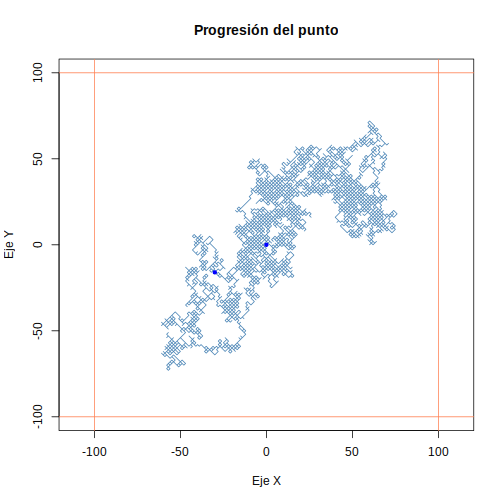
\includegraphics[width=\maxwidth]{figure/unnamed-chunk-4-1} 

}



\end{knitrout}
	
Atenci�n: Si en el directorio {\em figure} existe un archivo con el mismo nombre que el que se genera (aunque con otra extensi�n) puede dar problemas. Utilice un directorio vac�o.

Este es el histograma de $y$ (opciones de tama�o doble):

\begin{knitrout}
\definecolor{shadecolor}{rgb}{0.969, 0.969, 0.969}\color{fgcolor}\begin{kframe}
\begin{alltt}
    \hlkwd{hist}\hlstd{(y)}
\end{alltt}
\end{kframe}

{\centering 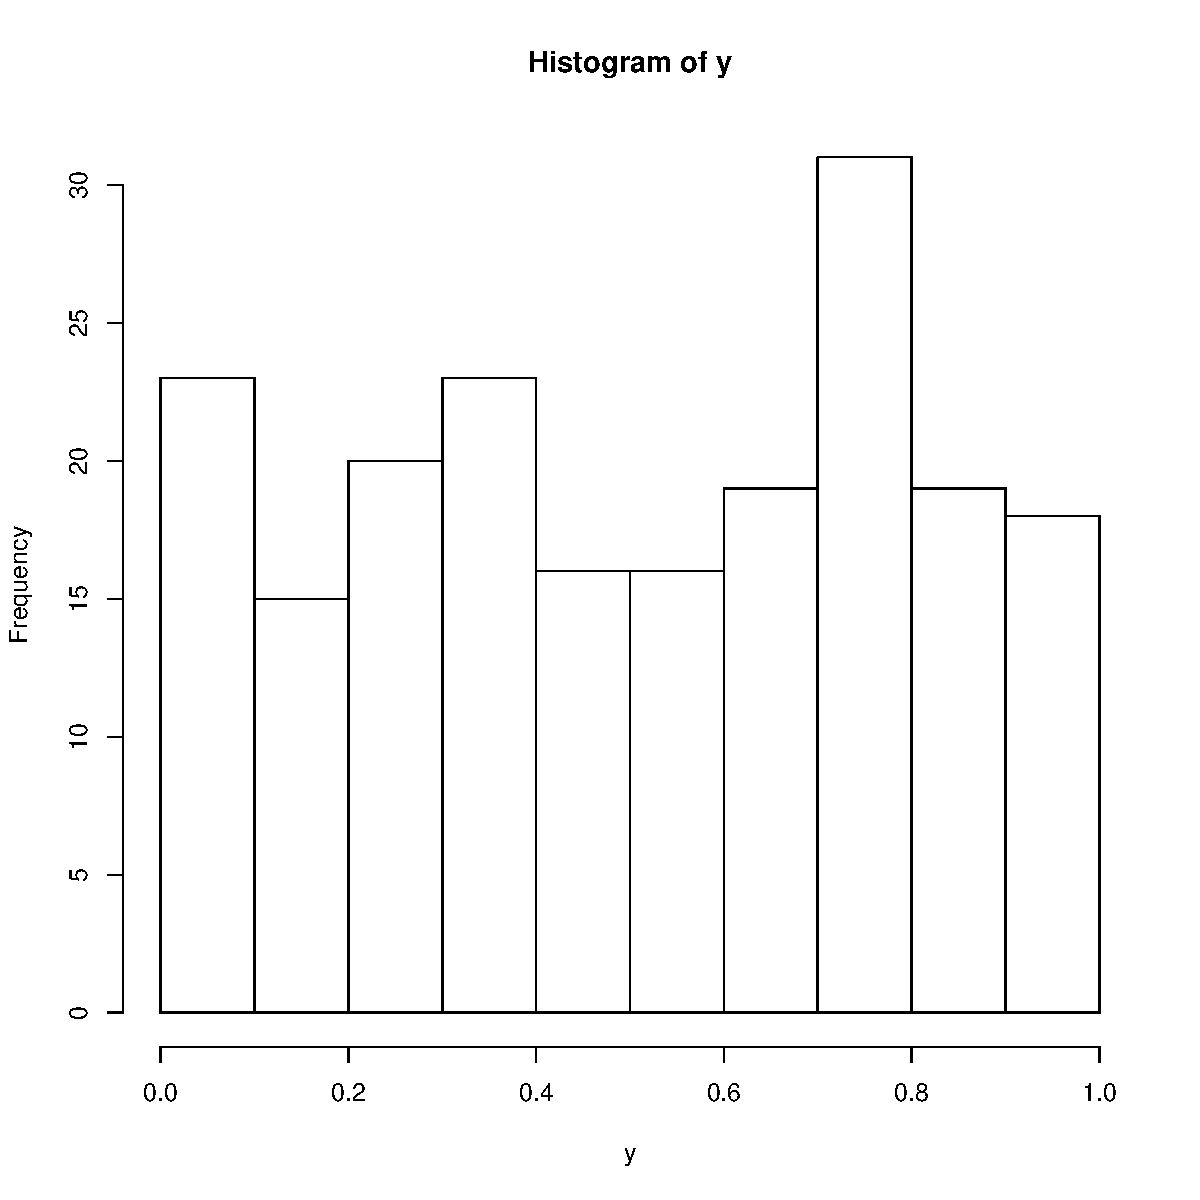
\includegraphics[width=\maxwidth]{figure/unnamed-chunk-5-1} 

}



\end{knitrout}
	

Puedo escribir resultados en la propia l�nea con la orden \code{Sexpr{}}, 
como por ejemplo la media de $x$ es  0.0203292 y la de de $y$ es  0.5060622.

Nota: Al finalizar compilo el archivo \LaTeX { } (extensi�n .tex) con la opci�n de paso directo a PDF. Evidentemente he instalado previamente un compilador de LaTeX, como, por ejemplo, MikTeX.
\end{document}
